\documentclass[aspectratio=169,10pt,handout]{beamer}
\usetheme[progressbar=frametitle,noslidenumbers]{metropolis}

% TU DORTMUND-LIKE FONT
\usepackage[no-math]{fontspec}
\setsansfont[
  Ligatures = TeX,
  BoldFont = FiraSans,
  ItalicFont = FiraSans-LightItalic,
  BoldItalicFont = FiraSans-Italic
]{FiraSans-Light}
\newfontfamily{\bxseries}{FiraSans-SemiBold}[
  LetterSpace=3.0,
  WordSpace=1.33,
  ItalicFont = FiraSans-SemiBoldItalic
]
\usefonttheme[onlymath]{serif}

% TIKZ AND COLOR
\usepackage{graphicx,color}
\DeclareGraphicsExtensions{%
    .pdf,.PDF,%
    .png,.PNG,%
    .jpg,.jpeg,.JPG,.JPEG}
\usepackage{tikz}
\usepackage{pgfplots}
\pgfplotsset{compat=1.15}
\usetikzlibrary{calc,patterns,shapes,positioning,arrows.meta,shapes.geometric}
\usetikzlibrary{decorations.pathreplacing}
\usepgfplotslibrary{fillbetween}

% color palette
\definecolor{tu01}{HTML}{84B818}
\definecolor{tu02}{HTML}{D18B12}
\definecolor{tu03}{HTML}{1BB5B5}
\definecolor{tu04}{HTML}{F85A3E}
\definecolor{tu05}{HTML}{4B6CFC}
\definecolor{tu06}{HTML}{E3B505}
\definecolor{tu07}{HTML}{AF331D}
\definecolor{tu08}{HTML}{000000}
\definecolor{tu09}{HTML}{AAAAAA}
\definecolor{tu10}{HTML}{444444}
\definecolor{tu11}{HTML}{84B818}

% mixed and light colors
\colorlet{tu01light}{tu01!40}
\colorlet{tu02light}{tu02!40}
\colorlet{tu03light}{tu03!40}
\colorlet{tu04light}{tu04!40}
\colorlet{tu05light}{tu05!40}
\colorlet{tu06light}{tu06!40}
\colorlet{tu07light}{tu07!40}
\colorlet{tu08light}{tu08!40}
\colorlet{tu09light}{tu09!40}
\colorlet{tu10light}{tu10!40}
\colorlet{tu11light}{tu11!40}

\colorlet{tu01midlight}{tu01!60}
\colorlet{tu02midlight}{tu02!60}
\colorlet{tu03midlight}{tu03!60}
\colorlet{tu04midlight}{tu04!60}
\colorlet{tu05midlight}{tu05!60}
\colorlet{tu06midlight}{tu06!60}
\colorlet{tu07midlight}{tu07!60}
\colorlet{tu08midlight}{tu08!60}
\colorlet{tu09midlight}{tu09!60}
\colorlet{tu10midlight}{tu10!60}
\colorlet{tu11midlight}{tu11!60}

\colorlet{tu01dark}{tu01!80!black}
\colorlet{tu02dark}{tu02!80!black}
\colorlet{tu03dark}{tu03!80!black}
\colorlet{tu04dark}{tu04!80!black}
\colorlet{tu05dark}{tu05!80!black}
\colorlet{tu06dark}{tu06!80!black}
\colorlet{tu07dark}{tu07!80!black}
\colorlet{tu08dark}{tu08!80!black}
\colorlet{tu09dark}{tu09!80!black}
\colorlet{tu10dark}{tu10!80!black}
\colorlet{tu11dark}{tu11!80!black}

\colorlet{tu01middark}{tu01!90!black}
\colorlet{tu02middark}{tu02!90!black}
\colorlet{tu03middark}{tu03!90!black}
\colorlet{tu04middark}{tu04!90!black}
\colorlet{tu05middark}{tu05!90!black}
\colorlet{tu06middark}{tu06!90!black}
\colorlet{tu07middark}{tu07!90!black}
\colorlet{tu08middark}{tu08!90!black}
\colorlet{tu09middark}{tu09!90!black}
\colorlet{tu10middark}{tu10!90!black}
\colorlet{tu11middark}{tu11!90!black}

\colorlet{verylightgray}{gray!3}
\colorlet{lightgray}{gray!25}
\colorlet{midlightgray}{gray!60}
\colorlet{anthracite}{black!85}

% aliases
\colorlet{tudo}{tu01}
\colorlet{tuorange}{tu02}
\colorlet{tudolight}{tu01light}
% 'axis line on top' option
\makeatletter \newcommand{\pgfplotsdrawaxis}{\pgfplots@draw@axis} \makeatother
\pgfplotsset{axis line on top/.style={
  axis line style = white,
  ticklabel style = white,
  tick style = white,
  axis on top = false,
  after end axis/.append code = {
    \pgfplotsset{
      axis line style = black,
      ticklabel style = black,
      tick style = black,
      grid = none
    }
    \pgfplotsdrawaxis
  }
}}

% elegant legend on the outside
\pgfplotsset{outside legend/.style = {
  legend style = {
    draw = none,
    fill = none,
    at = {(1.15,.5)},
    anchor = west,
    row sep = .25em,
    inner sep = 0pt
  }
}}

% default axis style
\pgfplotsset{default axis/.style = {
  axis line on top,
  axis line style = {anthracite, semithick},
  axis background/.style = {fill = white},
  legend cell align = {left},
  scaled y ticks = false
}}

\pgfplotsset{active axis/.style = {%
  default axis,
  reverse legend,
  legend cell align={left}
}}

% histograms
\pgfplotsset{histogram axis/.style = {
  default axis,
  legend style = {
    at = {(0.98,0.02)},
    anchor = south east
  },
  legend cell align = left
}}

\pgfplotsset{histogram plot/.style = {
  const plot,
  thick,
  mark = none
}}

% progress plots
\pgfplotsset{progress axis/.style = {
  default axis
}}

\pgfplotsset{progress plot/.style = {
  thick,
  solid,
  mark options = {
    scale = 1.5,
    fill = white,
    thick
  }
}}


\pgfplotsset{active plot/.style = {%
  mark = none
}}

\pgfplotsset{a00/.style = {active plot, gray}}
\pgfplotsset{a01/.style = {active plot, blue}}
\pgfplotsset{a02/.style = {active plot, green}}
\pgfplotsset{a03/.style = {active plot, red}}


% marks for progress plots
\pgfplotsset{m00/.style = {mark = none, anthracite, densely dashed}}
\pgfplotsset{m01/.style = {tu01midlight, mark = *,         every mark/.append style = {draw = tu01middark}, every error bar/.style = {color = tu01}}}
\pgfplotsset{m02/.style = {tu02midlight, mark = square*,   every mark/.append style = {draw = tu02middark}, every error bar/.style = {color = tu02}}}
\pgfplotsset{m03/.style = {tu03midlight, mark = triangle*, every mark/.append style = {draw = tu03middark}, every error bar/.style = {color = tu03}}}
\pgfplotsset{m04/.style = {tu04midlight, mark = diamond*,  every mark/.append style = {draw = tu04middark}, every error bar/.style = {color = tu04}}}
\pgfplotsset{m05/.style = {tu05midlight, mark = pentagon*, every mark/.append style = {draw = tu05middark}, every error bar/.style = {color = tu05}}}
\pgfplotsset{m06/.style = {tu06midlight, mark = otimes*,   every mark/.append style = {draw = tu06middark}, every error bar/.style = {color = tu06}}}
\pgfplotsset{m07/.style = {tu07midlight, mark = oplus*,    every mark/.append style = {draw = tu07middark}, every error bar/.style = {color = tu07}}}
\pgfplotsset{m08/.style = {tu08midlight, mark = star*,     every mark/.append style = {draw = tu08middark}, every error bar/.style = {color = tu08}}}
\pgfplotsset{m09/.style = {tu09midlight, mark = x,         every mark/.append style = {draw = tu09middark}, every error bar/.style = {color = tu09}}}
\pgfplotsset{m10/.style = {tu10midlight, mark = +,         every mark/.append style = {draw = tu10middark}, every error bar/.style = {color = tu10}}}
\pgfplotsset{m11/.style = {tu11midlight, mark = |,         every mark/.append style = {draw = tu11middark}, every error bar/.style = {color = tu11}}}
% also: 'asterisk', '-', and most of the above without '*'

% bar plots
\pgfplotsset{b01/.style={gray!40,every error bar/.style={opacity=1,thick,gray!80},mark=none,draw=none}}
\pgfplotsset{b02/.style={tu01midlight,postaction={pattern=crosshatch dots, pattern color=tu01middark},every error bar/.style={opacity=1,thick,tu01dark},mark=none,draw=none}}
\pgfplotsset{b03/.style={tu03midlight,postaction={pattern=north east lines,pattern color=tu03middark},every error bar/.style={opacity=1,thick,tu03dark},mark=none,draw=none}}
\pgfplotsset{b04/.style={tu02midlight,postaction={pattern=north west lines,pattern color=tu02middark},every error bar/.style={opacity=1,thick,tu02dark},mark=none,draw=none}}
\pgfplotsset{b05/.style={tu04midlight,postaction={pattern=crosshatch,pattern color=tu04middark},every error bar/.style={opacity=1,thick,tu04dark},mark=none,draw=none}}


\setbeamercolor{normal text}{fg=black} % black, not gray

% MARGINS FOR THE TIKZ OVERLAY
\newlength{\horizontalmargin}
\setlength{\horizontalmargin}{4mm}
\newlength{\verticalmargin}
\setlength{\verticalmargin}{3mm}
\newlength{\headerheight}
\setlength{\headerheight}{16mm}

\usepackage[super]{nth}

\title{Active Simulation Data Mining}
\subtitle{Workshop on Interactive Adaptive Learning at ECML-PKDD 2019}
\date{September \nth{16}, 2019}
\author{Mirko Bunse}
\institute{TU Dortmund, AI Group, 44221 Dortmund, Germany}
\titlegraphic{\hfill
\includegraphics[height=8mm]{img/logo_s876}}


\begin{document}


\begin{frame}{}
\begin{tikzpicture}[overlay, remember picture]

% boundary coordinates
\fill[white] (current page.north west) rectangle (current page.south east); % ensure a clear white background
\coordinate[shift={(+\horizontalmargin,-\verticalmargin)}] (page north west) at (current page.north west);
\coordinate[shift={(-\horizontalmargin,-\verticalmargin)}] (page north east) at (current page.north east);
\coordinate[shift={(+\horizontalmargin,+\verticalmargin)}] (page south west) at (current page.south west);
\coordinate[shift={(-\horizontalmargin,+\verticalmargin)}] (page south east) at (current page.south east);
% \draw[ultra thin, gray] (page north west) -- (page north east) -- (page south east) -- (page south west) -- cycle;

% style definitions
\tikzset{nosep/.style={inner sep=0pt, outer sep=0pt}}

% title
\tikzset{titlenode/.style={anchor=north west, nosep, text=white, scale=.92, transform shape}}
\fill[tu01] (current page.north west) rectangle ($(current page.north east) - (0mm,\headerheight)$);
\node[titlenode] (heading) at (page north west) {\bxseries\Large\strut ARIEL Discovery Challenge};
\node[titlenode] (authors) at (heading.south west)
  {\bfseries\normalsize\strut basel321 \hspace*{-1pt} (Mirko Bunse, \hspace*{-1pt} Lukas Heppe, \hspace*{-1pt} and Katharina Morik)};

% logos in footer
\node[anchor=south east, nosep, inner xsep=5pt, minimum height=10mm]
  (logo_s876) at (page south east) {
\includegraphics[height=9mm]{img/logo_s876}};
\node[anchor=south west, nosep, inner xsep=3pt, minimum height=10mm]
  (logo_tudo) at (page south west) {
\includegraphics[height=6mm]{img/logo_tudo}};

% coordinates bounding the content area
\coordinate (content north west) at ($(current page.north west) + (+\horizontalmargin,-\headerheight)$);
\coordinate (content north east) at ($(current page.north east) + (-\horizontalmargin,-\headerheight)$);
\coordinate (content south west) at (logo_tudo.north west);
\coordinate (content south east) at (logo_s876.north east);
\coordinate (content east) at ($(content north east) !.5! (content south east)$);
\coordinate (content north) at ($(content north east) !.5! (content north west)$);
\coordinate (content north west west) at ($(content north west) !.16! (content south west)$);
\coordinate (content south west west) at ($(content north west) !.92! (content south west)$);
% \draw[ultra thin, gray] (content north west) -- (content north east) -- (content south east) -- (content south west) -- cycle;

\node[anchor=north, align=center] (architecture) at ([yshift=-3mm] content north) {\parbox{.8\textwidth}{%
  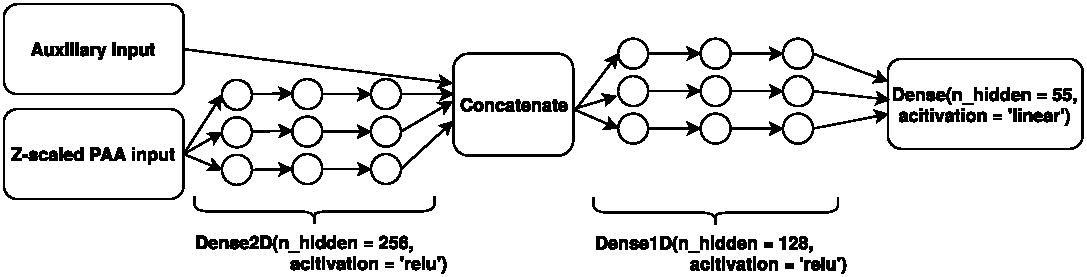
\includegraphics[width=.8\textwidth]{img/neural-network-architecture}
}};

\node[anchor=north, align=left, inner sep=2mm] at (architecture.south) {\parbox{\textwidth}{%
% - we used a deep dense(!) ReLu network with approx 1 Million parameters
% - we did NOT use the raw data, but a piecewise aggregate approximation (PAA) on Z-scaled time series,
%   reducing the number of time steps to only 30
% - however, we maintained the error of the Z scaling and the error of the PAA by computing the first
%   4 moments of the raw input and the reconstruction error of the PAA, so that no information is lost by these pre-processing steps.
% - we aggregate the predictions for each planet. There's 100 different instances for each of them,
%   but we already know that a planet observed with multiple noise instances is still the same planet with the same radii.
% - we use a bagging ensemble to get stable predictions, which is particularly important due to the weights used in your scoring function
%   (which we could not assess even approximately)
% - we did NOT use one of the auxiliary target variables
% - we did NOT use the final evaluation data in a transfer or semi-supervised style 
  \begin{itemize}
  	\item Deep Dense ReLu nets \, {\small with $\approx 10^6$ params}
  	\item Aggregate predictions for each planet \, {\small having 100 noise instances + bagging}
  	\item No additional targets
  	\item Not using the un-labeled data \, {\small to be predicted}
  \end{itemize}
}}; 

\end{tikzpicture}
\end{frame}


\begin{frame}{}
\begin{tikzpicture}[overlay, remember picture]

% boundary coordinates
\fill[white] (current page.north west) rectangle (current page.south east); % ensure a clear white background
\coordinate[shift={(+\horizontalmargin,-\verticalmargin)}] (page north west) at (current page.north west);
\coordinate[shift={(-\horizontalmargin,-\verticalmargin)}] (page north east) at (current page.north east);
\coordinate[shift={(+\horizontalmargin,+\verticalmargin)}] (page south west) at (current page.south west);
\coordinate[shift={(-\horizontalmargin,+\verticalmargin)}] (page south east) at (current page.south east);
% \draw[ultra thin, gray] (page north west) -- (page north east) -- (page south east) -- (page south west) -- cycle;

% style definitions
\tikzset{nosep/.style={inner sep=0pt, outer sep=0pt}}

% title
\tikzset{titlenode/.style={anchor=north west, nosep, text=white, scale=.92, transform shape}}
\fill[tu01] (current page.north west) rectangle ($(current page.north east) - (0mm,\headerheight)$);
\node[titlenode] (heading) at (page north west) {\bxseries\Large\strut ARIEL Discovery Challenge};
\node[titlenode] (authors) at (heading.south west)
  {\bfseries\normalsize\strut basel321 \hspace*{-1pt} (Mirko Bunse, \hspace*{-1pt} Lukas Heppe, \hspace*{-1pt} and Katharina Morik)};

% % logos in footer
% \node[anchor=south east, nosep, inner xsep=5pt, minimum height=10mm]
%   (logo_s876) at (page south east) {
\includegraphics[height=9mm]{img/logo_s876}};
% \node[anchor=south west, nosep, inner xsep=3pt, minimum height=10mm]
%   (logo_tudo) at (page south west) {
\includegraphics[height=6mm]{img/logo_tudo}};

% coordinates bounding the content area
\coordinate (content north west) at ($(current page.north west) + (+\horizontalmargin,-\headerheight)$);
\coordinate (content north east) at ($(current page.north east) + (-\horizontalmargin,-\headerheight)$);
\coordinate (content south west) at (logo_tudo.north west);
\coordinate (content south east) at (logo_s876.north east);
\coordinate (content east) at ($(content north east) !.5! (content south east)$);
\coordinate (content north) at ($(content north east) !.5! (content north west)$);
\coordinate (content north west west) at ($(content north west) !.16! (content south west)$);
\coordinate (content south west west) at ($(content north west) !.92! (content south west)$);
% \draw[ultra thin, gray] (content north west) -- (content north east) -- (content south east) -- (content south west) -- cycle;

\node[anchor=north west, align=center] (score) at ([yshift=-5mm] content north west) {\parbox{.9\textwidth}{%
  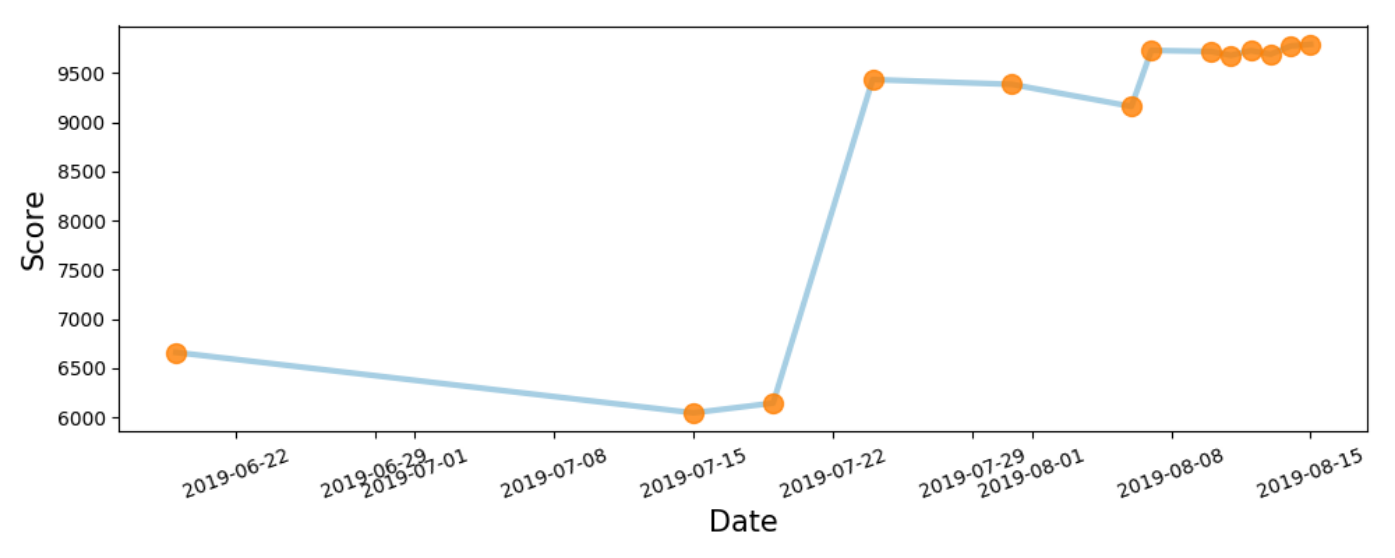
\includegraphics[width=.9\textwidth]{img/score}
}};

\draw[tu02, very thick, rounded corners] ($(score.north west) !.53! (score.north east)$) rectangle ($(score.south west) !.65! (score.south east)$);
\node[anchor=north, inner sep=2mm, font=\bxseries, text=tu02] at ($(score.south west) !.59! (score.south east)$) {PAA};

\draw[tu02, very thick, rounded corners] ($(score.north west) !.78! (score.north east)$) rectangle ($(score.south west) !.84! (score.south east)$);
\node[anchor=north, inner sep=2mm, font=\bxseries, text=tu02] at ($(score.south west) !.81! (score.south east)$) {Bagging};

\draw[tu01, very thick] ([xshift=-6mm]$(score.north east) !.1! (score.south east)$) -- node[pos=1, anchor=west, inner sep=2mm, font=\bxseries] {9795.0 (\nth{5})} ++(8mm,0mm);

\end{tikzpicture}
\end{frame}


\end{document}